\chapter{Create groups of layers}

\pagestyle{fancy}
\fancyhf{}
\fancyhead[OC]{\leftmark}
\fancyhead[EC]{\rightmark}
%\renewcommand{\footrulewidth}{1pt}
\cfoot{\thepage}

%%%%%%%%%%%%%%%%%%%%%%%%%%%%%%%%%%%%%%%%%%%%%%%%%%%%%%%%%%%
%%%%%%%%%%%%%%%%%%%%%%%%%%%%%%%%%%%%%%%%%%%%%%%%%%%%%%%%%%%

\section{Set up a group}

We now have multiple layers that contain the same data but with different symbology, some of your layers may be opaque. Having more than one of these selected is not useful. We can set up groups within the \textit{Layers Panel} so that the layers within the group are mutually exclusive.\\
%In our example, we now have two layers that are opaque. Having both selected at once is not useful. We can set up groups within the \textit{Layers Panel} so that the layers within the group are mutually exclusive.\\

At the top of the \textit{Layers} Panel, select \textit{Add Group} 
	\begin{tabular}{@{}c@{}}
\includegraphics[width=4ex]{images/add_group_icon.png}\end{tabular}
(and rename the group: "stop\_search\_layers").\\
This will add a group within the \textit{Layers} panel. Drag and drop the layers into the group.\\
Right click on the group name within the \textit{Layers} Panel and select \textit{Mutually Exclusive Group}.\\
Make sure the base map is still at the bottom of the list of layers.

\begin{figure}[!h]
	\centering
	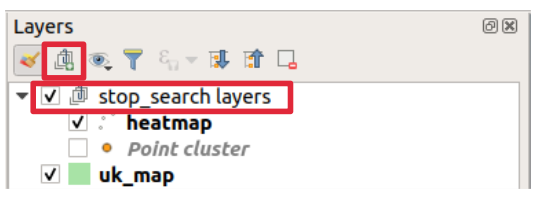
\includegraphics[width=0.4\textwidth]{images/group_layers1.png}
	\caption{Create a group, then drag and drop the relevant layers in}
	\label{ft_fig_firstfig3}
\end{figure}
